\chapter{Results \& Discussion}

In this chapter we will present and discuss the relevant outputs of our RNA-seq pipeline, and the reasoning behind our chosen approach, with accordance to the project's aim and objectives (\autoref{Aim and Objectives}). As described thoroughly in \autoref{pipeline}, we have:

\begin{itemize}
\item Performed QC checks on the four raw FASTQ files, and filtered out data with signs of poor quality.
\item Aligned the reads to the GRCh38.p13 reference genome, excluding reads with ambiguous mapping, to produce gene-centric read count matrices.
\item Filtered genes with low counts (<10), as these would be indistinguishable from noise.
\item Normalised the read counts for biologically irrelevant extraneous variables between the libraries using the \ac{TMM} method.
\item Quantified the magnitude and significance of the differences in gene expression between the treated samples and the control. These were represented as the \ac{logFC} and \textit{p}-values respectively, given for each gene and stored in a data frame.
\item Adjusted the \textit{p}-values for multiple-testing, converting them to \ac{FDR}s with the Benjamini-Hochberg controlling procedure.
\item Set an \ac{FDR} cut-off of 0.05 and a \ac{logFC} cut-off of 1.5 to define which genes are truly differentially expressed.
\item Annotated the \ac{DEG}s and performed Gene Set Enrichment Analysis to put them into their biological context.
\end{itemize}


\section{Determining the Optimal Tools}
\label{determining tools}

Before we begin tackling the pipeline, we should first explain the reasoning behind the choices of its constituent tools. This will make heavy use of the literature reviewed in Section \ref{Computational Tools}, through which we will achieve this project's first objective. Extensive descriptions of the final tools implemented in the pipeline can be found throughout Section \ref{RNA-seq: in silico}.
% NOTE SEE IF U NEED TO CHANGE THIS. Maybe group all the tools in a single place

Tools which measure quality metrics without altering the data require little justification for their use, their mention occasionally being completely omitted from RNA-seq studies (\autoref{tab:rnaseq_experiments}). \textbf{FastQC} provides a detailed analysis of the contents of FASTQ files and highlights indications of low quality reads. While FastQC results are detailed, they lack the detection of external nucleotide contaminants in the data. This information was supplemented with the results from \textbf{FastQScreen} which aligns the experimental sequences to common contaminant sequences (e.g. mouse, \textit{Drosophila}, rRNA) and provides a graph marking any successful alignments. \textbf{MultiQC} is a staple of sequencing data quality control, unparalleled in its ability to combine logs from a wide range of supported tools and across multiple samples. This greatly facilitates cross-sample comparisons.

\cite{he2020assessing} found that the effects of their tested preprocessing techniques on downstream analyses are marginal, thus we base our decision on the frequency of the tools used in tables \ref{tab:rnaseq_experiments} and \ref{tab:packaged_pipelines} and their functionality. \textbf{Cutadapt} adequately satisfies these criteria, providing the means to trim adapter sequences and remove short reads. \textbf{Trim Galore!} pipes the output to FastQC, which facilitates the reassessment of quality. To complement their functionality, \textbf{Prinseq++} was chosen to detect and remove regions of low-complexity which were noticeably neglected in studies' preprocessing steps. 
%\cite{liao2020read} and \cite{he2020assessing} doubt the necessity of trimming at all.

Despite \textbf{STAR} being demanding of RAM \citep{Dobin2013} and slower than more light-weight aligners \citep{srivastava2020alignment}, these were not limiting factors due to our access to a High Performance Computer (HPC) and small number of samples. \cite{srivastava2020alignment} found that the choice between quasi-mappers (e.g. Salmon) and traditional aligners (e.g. STAR) is a trade-off between speed and accuracy. Similarly \cite{Zhang2017} found that pseudo-aligners Salmon and Kallisto require less runtime while maintaining similar accuracy to STAR. \cite{Schaarschmidt2020} find that the effect aligners have on the final list of \ac{DEG}s is negligible, and that all tested aligners can be used equally for RNA-seq. Even if STAR provides even a marginal increase in accuracy over quasi-aligners, this is preferable over any improvements in speed or computational demand provided by other aligners.

An RNA-seq quantification tool benchmark, \cite{teng2016benchmark}, conclude that their tested tools performed similarly, with the exception of the under-performing Flux Capacitor \citep{} and eXpress \citep{}. \textbf{RSEM} was amongst these tools, and was ultimately chosen on the basis of its statistical techniques based on \cite{li2010rna} to mitigate ambiguous read alignment. Its support for the STAR aligner is also convenient, allowing the combination of alignment and quantification steps. 

The choice of tools for downstream analyses was more complex, and deservent of their own subsections as follows.


\subsection{Adapting DGE Analysis to a Lack of Replicates}
\label{DGE no replicates}

The most difficult and time-consuming decision to make was the choice of tool to perform \ac{DGE} analysis. The invested effort was justified by the findings of \cite{williams2017empirical}, which state that the method of \ac{DGE} exhibits the strongest impact on the results out of all stages of the pipeline. Our data consists of three time points (1hr, 6hr, 12hr) and a negative control, each lacking replicates. 

Technical replicates allow the isolation of the non-biological variation to evaluate the quality of the instruments and methodology used. By contrast, biological replicates originate from different biological sources and are meant to test the biological variance of the samples. \cite{liu2014rna} find that in RNAseq biological variation is by far more important, and given a choice between the two, the researcher should invest in biological replicates. \cite{bullard2010evaluation} confirm this claim, finding that technical variation in RNAseq experiments is minimal. \cite{schurch2016many} found that using three biological replicates gave 20\% to 40\% of the \ac{DEG}s (varies according to the tool) compared to a full set of 42 replicates (representing the 'true' population). This rises to >85\% when considering genes with a log$_2$ fold change of >2. \cite{schurch2016many} state that ideally an RNAseq experiment for \ac{DGE} should have a minimum of six replicates per condition for all experiments and 12 replicates for experiments where the identification of \textit{all} the \ac{DEG}s, even the lowly expressed ones, is important. 

However, in practice, performing an experiment with large numbers of replicates is not always possible. Budget constraints and the still-high cost of sequencing are a common issue in RNAseq experiments. One may argue that this issue is mitigated due to the negligible technical variance of RNA-seq \citep{bullard2010evaluation} and the minimal biological variance in samples from the same \ac{ATRA}-resistant HL-60 cell line. In spite of this, the statistical tests used by conventional \ac{DGE} tools are dependent on the calculation of the variance or dispersion, which is not mathematically possible with a single reading per condition. To make the most of such datasets, several \ac{DGE} tools advertise their ability to work with just a single reading per experimental condition \citep{feng2012gfold, gim2016lpeseq, anders2010differential, wang2010degseq, al2014bootstrap}. Notably, DESeq2 does not support datasets without replicates. There is an unfortunate lack of review papers and independent studies which benchmark these tools. For this reason this section will be reviewing the available tools adapted to performing \ac{DGE} without replicates.

The first tool in this review will be \textbf{GFOLD} \citep{feng2012gfold}, developed specifically for datasets lacking in replicates. The developers acknowledge the dependence of \textit{p}-values on variance estimation, which is impossible without replicates. A unique GFOLD value replaces the standard metrics of significance (\textit{p}-values) and expression change (log$_2$ fold changes). \cite{feng2012gfold} describe the value as a relative change of the expression level. GFOLD is unique in that it is the only tool in this comparison that is called through the Linux command line, instead of being an R library.

\textbf{LPESeq} \citep{gim2016lpeseq} introduces the Local-Pooled-Error (LPE) method for few or single-replicate \ac{DGE} analysis. This method attempts to estimate transcript-specific variance using the raw values of each transcript per condition. Hypothesis testing for significant difference is then performed to identify the differentially expressed genes.

\textbf{IsoDE} \citep{al2014bootstrap} is a non-parametric method (i.e. it assumes no statistical distribution) and is based on bootstrapping. The algorithm generates FPKM estimates from read counts of each condition which undergo pairwise comparison.

An MA-plot-based method, the R library \textbf{DEGseq} \citep{wang2010degseq} (not to be confused with DESeq) accepts input .bed or .eland input files and outputs an XHTML page with \textit{p}-values, gene expression values and expression differences in the form of Q-values.

The final tool in this review is the Bioconductor R library \textbf{edgeR} \citep{edger}. It may be more accurately described as a collection of methods, neither of which are specifically adapted to data without replicates, but its documentation provides recommendations to adapt the analysis to such a situation. EdgeR and its normalisation technique TMM have already been covered extensively in Section \ref{EdgeR} and Section \ref{TMM} respectively. 

The lesser-known tools (GFOLD, LPESeq, DEGseq, IsoDE), while developed specifically to function without replicates, were found to be limited in functionality in comparison to \textbf{edgeR}. Additionally, due to their rather unconventional approach to \ac{DGE}, their output was found to be incompatible with other downstream libraries, limiting the potential for data exploration. 

EdgeR has multiple methods to determine which genes are differentially expressed (\autoref{edger_dge_options}). The likelihood ratio tests \citep{mccarthy2012differential} compared values against their mean, which was not applicable to our study as we needed to compare reads from treated cells against reads from untreated cells. Quasi-likelihood F-tests \citep{lun2016s, lund2012detecting} were simply not compatible to datasets lacking replicates. This leaves us with the \textit{classic} approach: the exact test for the negative binomial distribution \citep{robinson2007moderated, robinson2008small}. This is a pairwise test which compares the means between two groups of counts, applicable to experiments with a single factor. It should not be confused with Fisher's exact test \citep{fisher1922interpretation}, although the two share a number of similarities \citep{chen2014edger}.

The exact test for the negative binomial distribution still involves the calculation of dispersion of the data, but the edgeR vignette suggests a method to circumvent this. It suggests nominal values for the biological variation (\ac{BCV}) of our data based on previous experiments, from which we may derive an estimation for the dispersion. The vignette emphasises that this method is still inaccurate, but was deemed as the best possible solution given our data and the aforementioned potential techniques. By extension, the normalisation method native to edgeR, \textbf{TMM}, will be used to ensure proper function of the library.
% really perfect paper https://www.ncbi.nlm.nih.gov/pmc/articles/PMC4878611/#:~:text=Recommendations%20for%20RNA%2Dseq%20experiment%20design&text=At%20least%20six%20replicates%20per,all%20DE%20genes%20is%20important.

\subsection{Gene Set Analyses}

For further analyses on a gene-set level (e.g. involving \ac{GO} terms or \ac{KEGG} pathways), we must consider three main approaches described by \cite{khatri2012ten} and \cite{alhamdoosh2017combining}, ranked in order of increasing complexity: Over-Representation Analysis (\ac{ORA}), Gene Set Enrichment Analysis (\ac{GSEA}) and Pathway Topology Analysis (\ac{PTA}). More complex analyses with more factors implies greater accuracy, and \cite{nguyen2019identifying} confirms this intuition, showing that \ac{PTA} methods perform the best as they take into account the interactions between gene products, and the nature of their interaction (e.g. activation or inhibition). Conversely, the more complex the process, the harder it is for researchers to truly understand the underlying mechanisms and risk applying them incorrectly. A presentation by Pietrosemoli and Legendre\footnote{\url{https://ressources.france-bioinformatique.fr/sites/default/files/4\%20-\%20FGSA_Roscoff.pdf} (Last accessed 07/07/22)} references the principal of Occam’s Razor, which states that solutions should not be complicated beyond necessity. \cite{albert2020biostar} agrees that rather than believing that a 'black box' will work as one would wish, the researcher might prefer to use slightly simpler but comprehensible techniques.

For this project, \ac{GSEA} tools were chosen as a compromise between risk of human error and statistical accuracy, as a balance between these two philosophies. For this project we have chosen \textbf{GAGE} as the specific library that will generate the gene-set-level statistics to check which gene sets are differentially expressed. EdgeR has its own inbuilt gene set analysing functions, \texttt{goana} and \texttt{kegga}, however these only test for over-representation. This means that the analysis excludes important factors such as \ac{logFC}s and \textit{p}-values, and fails to output the direction of regulation of the gene set.
%Pathview?

\section{Read Quality Control}

This section encompasses all QC measures taken prior to quantification of the reads. MultiQC is able to read and compile log files from FastQC, FastQScreen, Cutadapt and STAR into a single interactive HTML file, allowing quality comparisons across samples. Figures \ref{fig:fastqc-status-check-heatmap} through \ref{fig:star_alignment_plot} are graphs downloaded directly from MultiQC.


\subsection{Assessing the Quality of the Raw Data}
\label{Assessing the Quality of the Raw Data}
We started off with four single-ended 50bp FASTQ files, one per experimental time point (control, 1hr, 6hr, 12hr), which were sequenced using the Illumina Stranded mRNA-seq workflow \citep{HiSeq2000}. Paired-end reads of a longer length would have been more accurate, although on their website\footnote{\url{https://emea.illumina.com/science/technology/next-generation-sequencing/plan-experiments/read-length.html} (Last accessed 16/06/22)}, Illumina suggests that single-ended 50bp reads suffice for a \ac{DGE} RNA-seq experiment.

\autoref{fig:fastqc-status-check-heatmap} shows the FastQC results for each raw file, summarised as a heatmap generated by MultiQC. Caution should be exercised when interpreting RNA data through FastQC, as the program is primarily calibrated to DNA data. Two modules failed consistently throughout the four samples received. This is normal and expected even for high-quality RNA \citep{hansen2010biases}. The failure of the \textit{Per base sequence content} module can be explained by a benign artefact of the random hexamer priming that occurs during library preparation, where the first 10-15 bases of RNA reads are non-uniformly enriched \citep{hansen2010biases}. The failure for the second module, textit{Sequence Duplication Levels} is explained by \autoref{fig:fastqc_sequence_duplication_levels_plot} and the text preceding it.

All four samples had <0.3\% \textit{N}-content on average on the first base of the reads and <0.1\% on the rest of the read, which the algorithm deems as good quality. All sequences of all samples had a single length of 51bp with <1\% overrepresented sequences and <0.5\% adapter contamination.

%Write about terminator caps in intro

% https://hbctraining.github.io/Intro-to-rnaseq-hpc-salmon/lessons/qc_fastqc_assessment.html
% Really good resource on RNAseq QC
 %Another one: https://rtsf.natsci.msu.edu/genomics/tech-notes/fastqc-tutorial-and-faq/#:~:text=FastQC%2C%20written%20by%20Simon%20Andrews,on%20a%20sequence%20data%20set.


% INTERNPRETING FASTQC REPORT NOTES:
% Real good resource of possible explanations:
% We have positional sequence bias: https://sequencing.qcfail.com/articles/positional-sequence-bias-in-random-primed-libraries/
% High Sequence Duplication levels are expected: https://www.biostars.org/p/307361/
%From Molecular Biology assignment:
%  One cycle per base pair would have been needed, so 50 cycles should have been performed.


\newpage
\begin{figure}[!h]
    \centering
    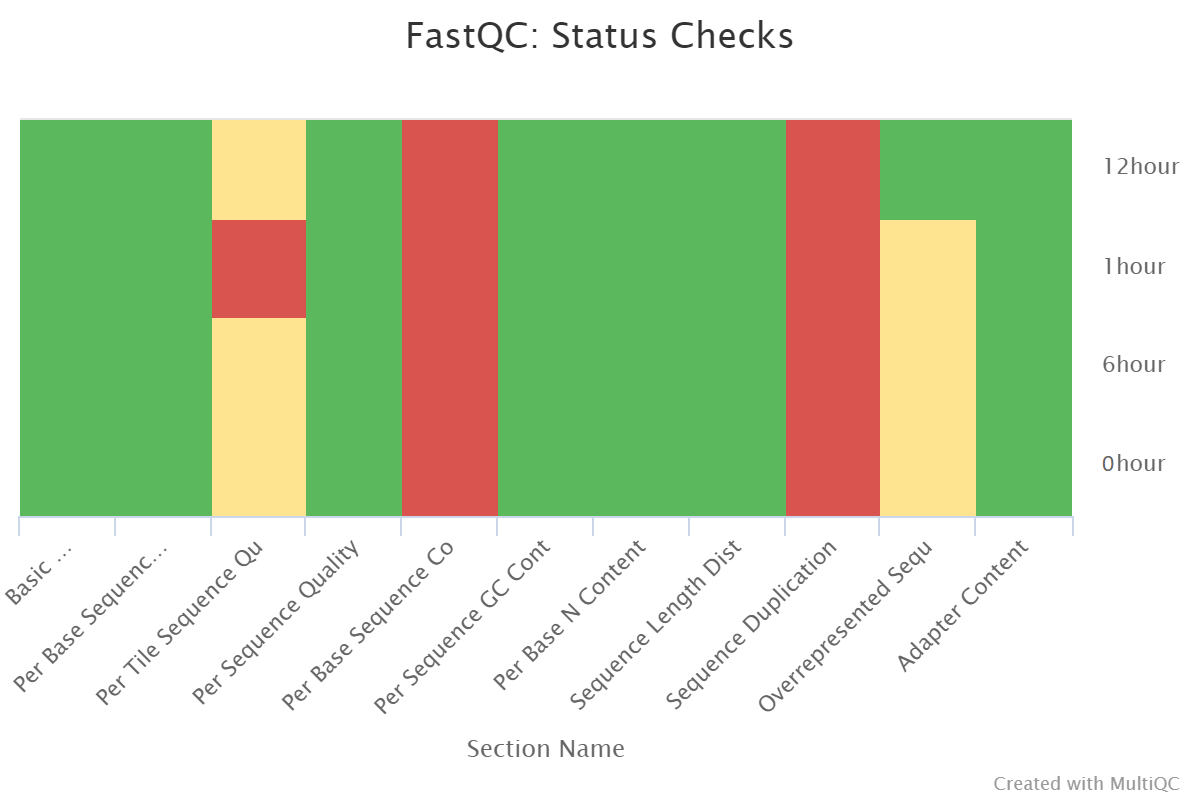
\includegraphics[width=1\textwidth]{fastqc-status-check-heatmap}
    \caption[Heat map showing the status of each FastQC module]{Heat map generated by MultiQC showing the status of each FastQC module: Pass, Warning or Fail.} 
    \label{fig:fastqc-status-check-heatmap}
\end{figure}

\newpage
Part of the sequencing process involved PCR amplification of cDNA, although not all sequences are amplified equally \citep{kozarewa2009amplification}. These PCR duplicates differ from 'natural' duplicates, i.e. those that originated from different mRNA molecules. Both these factors contribute to certain sequences being disproportionately abundant (as seen in \autoref{fig:fastqc_sequence_duplication_levels_plot}), which FastQC flags as duplicates, causing the failure of the \textit{Sequence Duplication Levels} module. \cite{parekh2016impact} state that there is no clear consensus on what should be done with these duplicates, with their removal producing conflicting results.

\begin{figure}[!h]
    \centering
    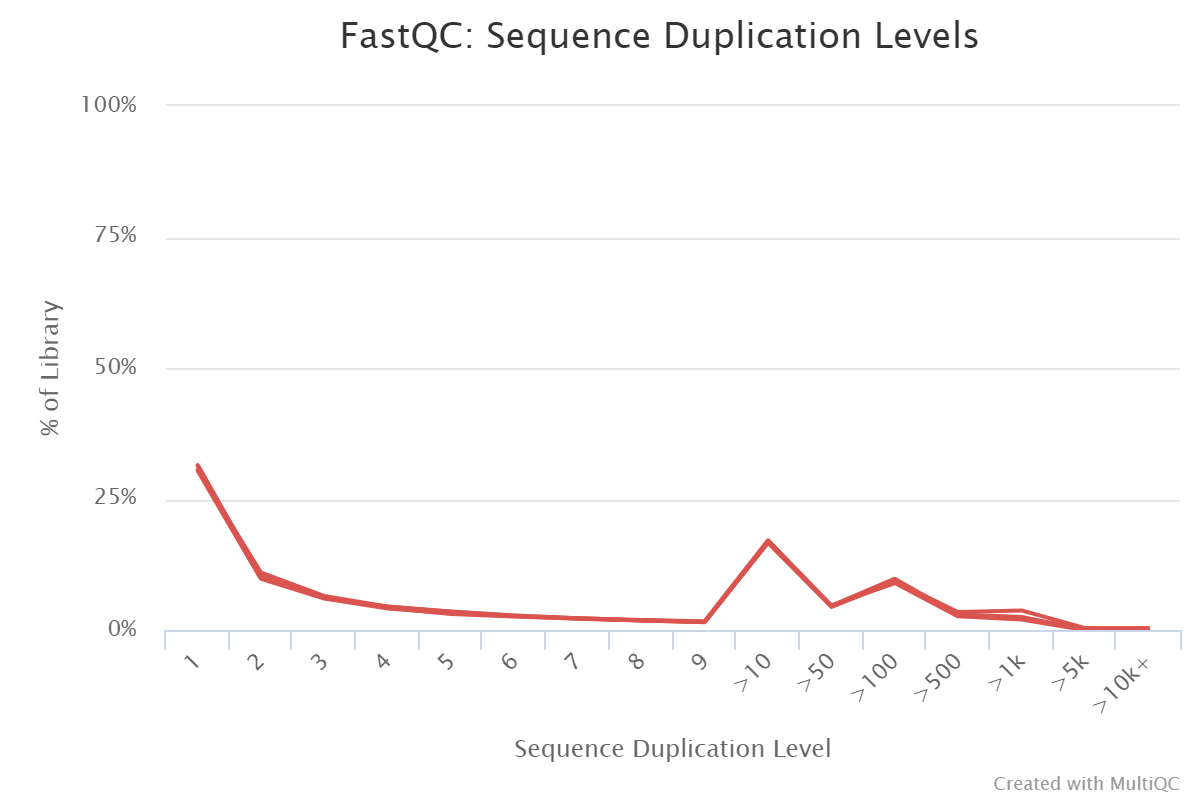
\includegraphics[width=1\textwidth]{fastqc_sequence_duplication_levels_plot}
    \caption[Sequence duplication levels plots for all samples]{Sequence duplication levels plots for all samples, showing the wide range of possible coverages in RNA data, ranging from 1 to >10,000.} 
    \label{fig:fastqc_sequence_duplication_levels_plot}
\end{figure}

\newpage
In Figure \ref{fig:fastqc_per_base_sequence_quality_plot}, sequence quality peaks at around the 14th base-pair, then gradually declines which is a classic sign of phasing. \cite{pfeiffer2018systematic} describe it as two similar phenomena: pre-phasing and post-phasing, both of which cause the reads to become out-of-sync. Pre-phasing occurs when two or more nucleotides bind to the read in a single cycle, causing the sequence to ‘skip’ a nucleotide. This often occurs when the flow-cell is not flushed properly or in the case of a defect terminator cap. Post-phasing is caused by the incomplete removal of the terminator cap, leading to the sequence lagging behind the rest of the cluster. As the number of cycles increases, the higher the probability of an error to occur which causes the read to become out of phase, and when this occurs, it will pollute the light signals of all subsequent cycles.


\begin{figure}[!h]
    \centering
    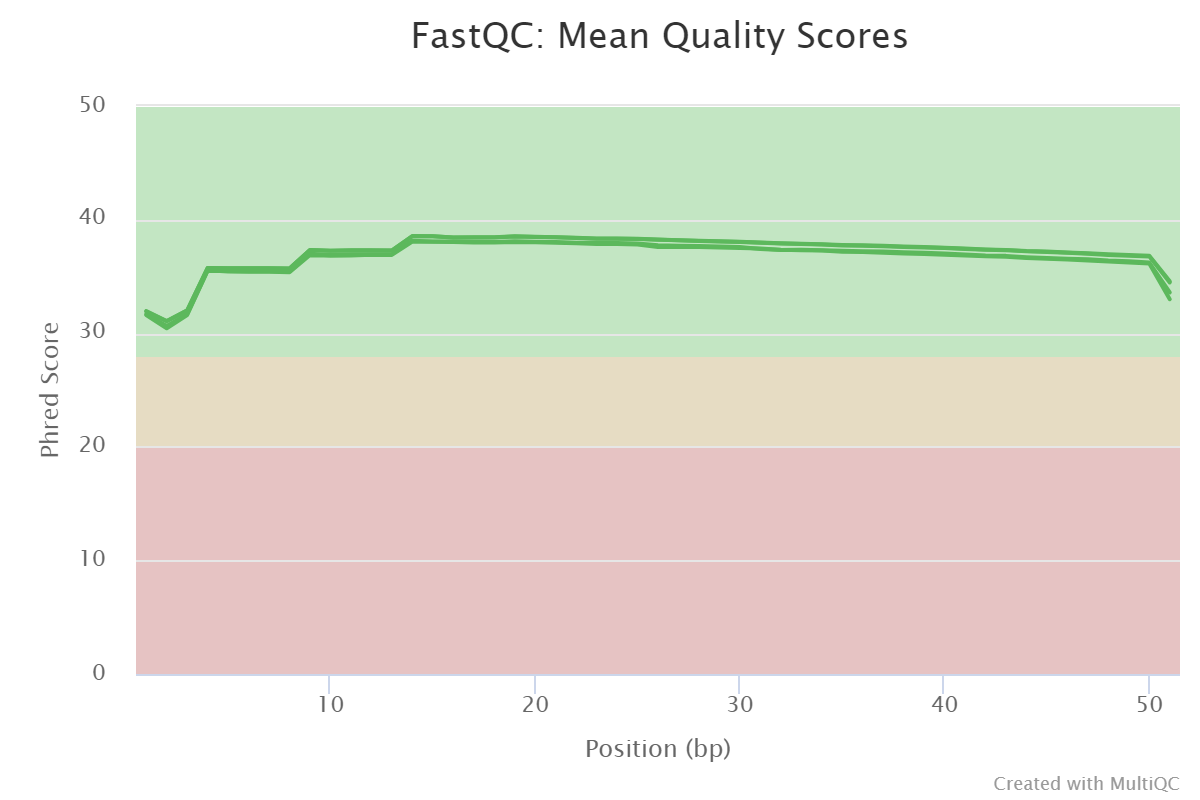
\includegraphics[width=1\textwidth]{fastqc_per_base_sequence_quality_plot}
    \caption{The aggregated mean Phred scores at each position of the reads.} % write about tpical pattern
    \label{fig:fastqc_per_base_sequence_quality_plot}
\end{figure}

\newpage
\autoref{fig:fastqc_per_sequence_gc_content_plot} shows a normal distribution which peaks around 48 \%GC, which is within the expected range for a human genome \citep{meunier2004recombination}. During PCR, endonucleases are less likely to cleave GC base pairs for two reasons: their triple bond, which is stronger than the double bond in AT pairs, and because of  a phenomenon called base stacking which contributes to its structural stability \citep{yakovchuk2006base}. This may lead to GC-bias \citep{benjamini2012summarizing}, although this does not seem to be present.

\begin{figure}[!h]
    \centering
    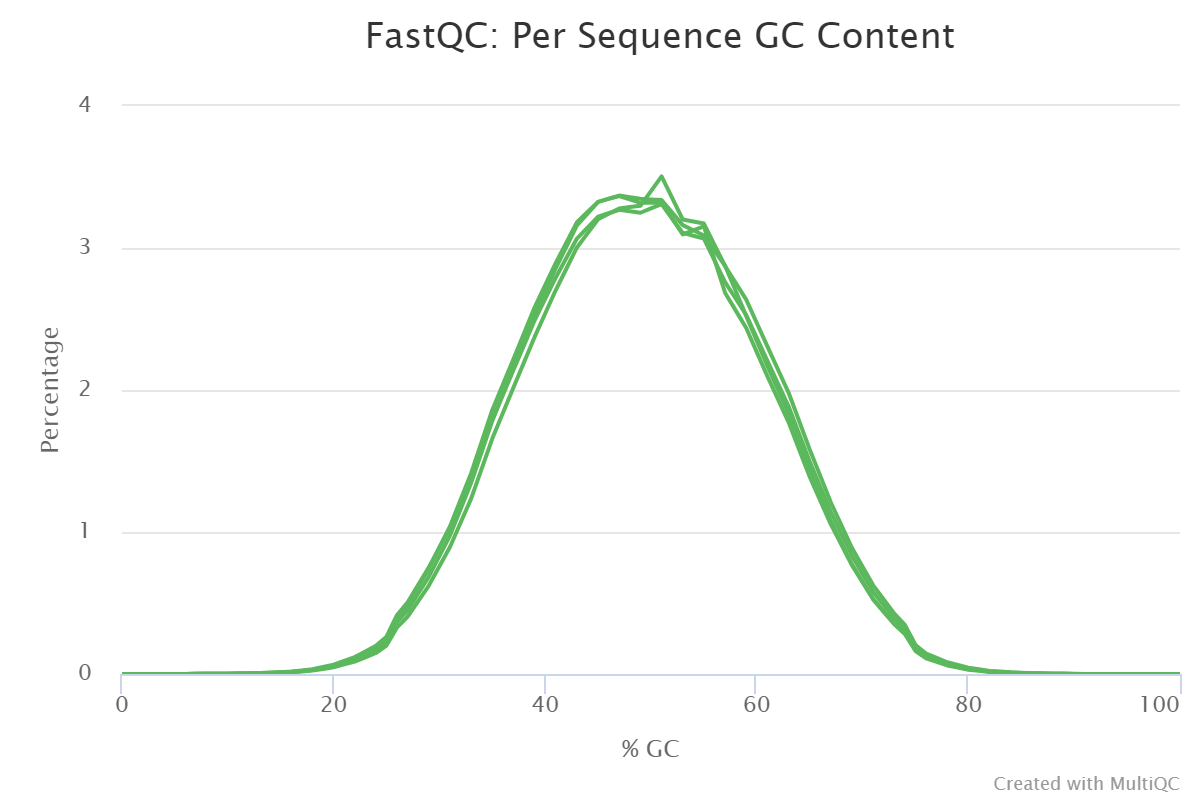
\includegraphics[width=1\textwidth]{fastqc_per_sequence_gc_content_plot}
    \caption{The distribution of GC percentages across the reads.}
    \label{fig:fastqc_per_sequence_gc_content_plot}
\end{figure}

\newpage
\autoref{fig:fastqc_per_sequence_quality_scores_plot} is similar to  \autoref{fig:fastqc_per_base_sequence_quality_plot}, except showing \textit{average} Phred scores on a sequence-level, instead of a base pair-level. The Phred score distribution is as expected for good quality data.


\begin{figure}[!h]
    \centering
    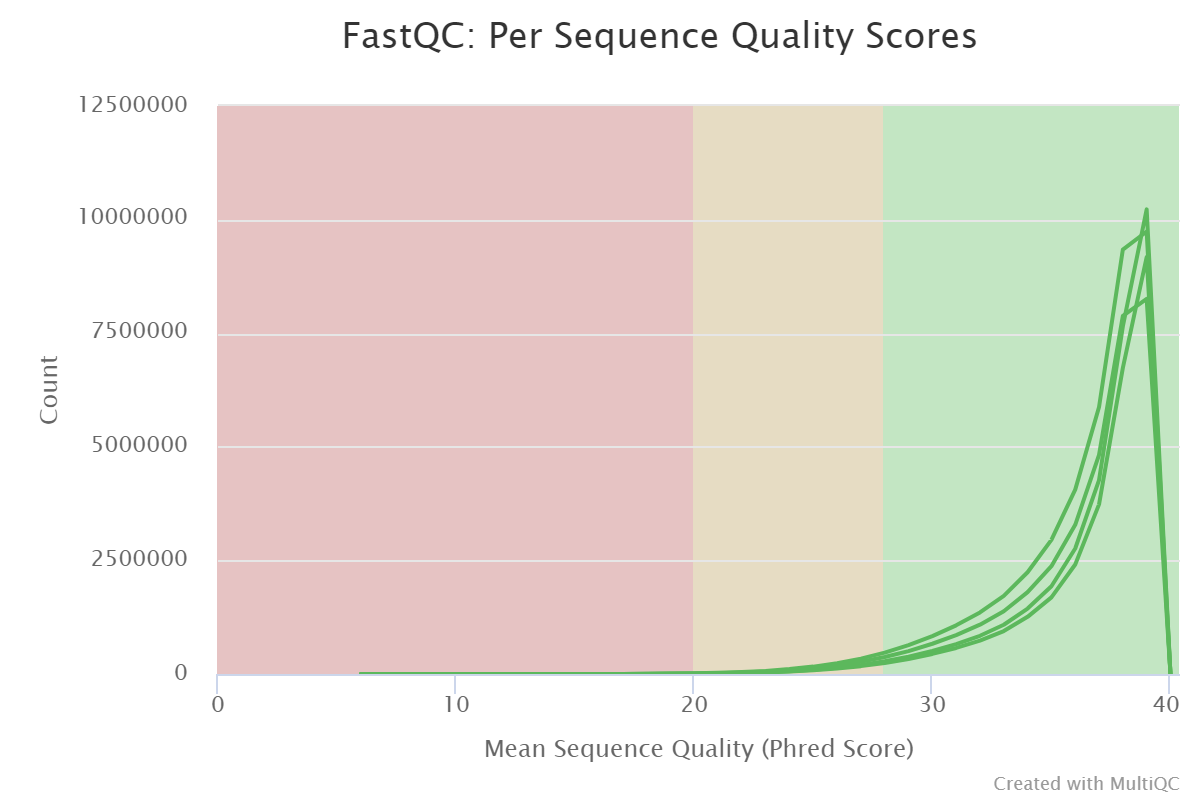
\includegraphics[width=1\textwidth]{fastqc_per_sequence_quality_scores_plot}
    \caption{The distribution of mean Phred scores across the reads.} % write about tpical pattern
    \label{fig:fastqc_per_sequence_quality_scores_plot}
\end{figure}

\newpage
Unequal read counts for each sample, as shown in \autoref{fig:fastqc_sequence_counts_plot} are expected in RNA-seq and adjusted for in the downstream pipeline. As previously stated, the presence of duplicate reads is relatively benign in RNA-seq \citep{parekh2016impact}.

\begin{figure}[!h]
    \centering
    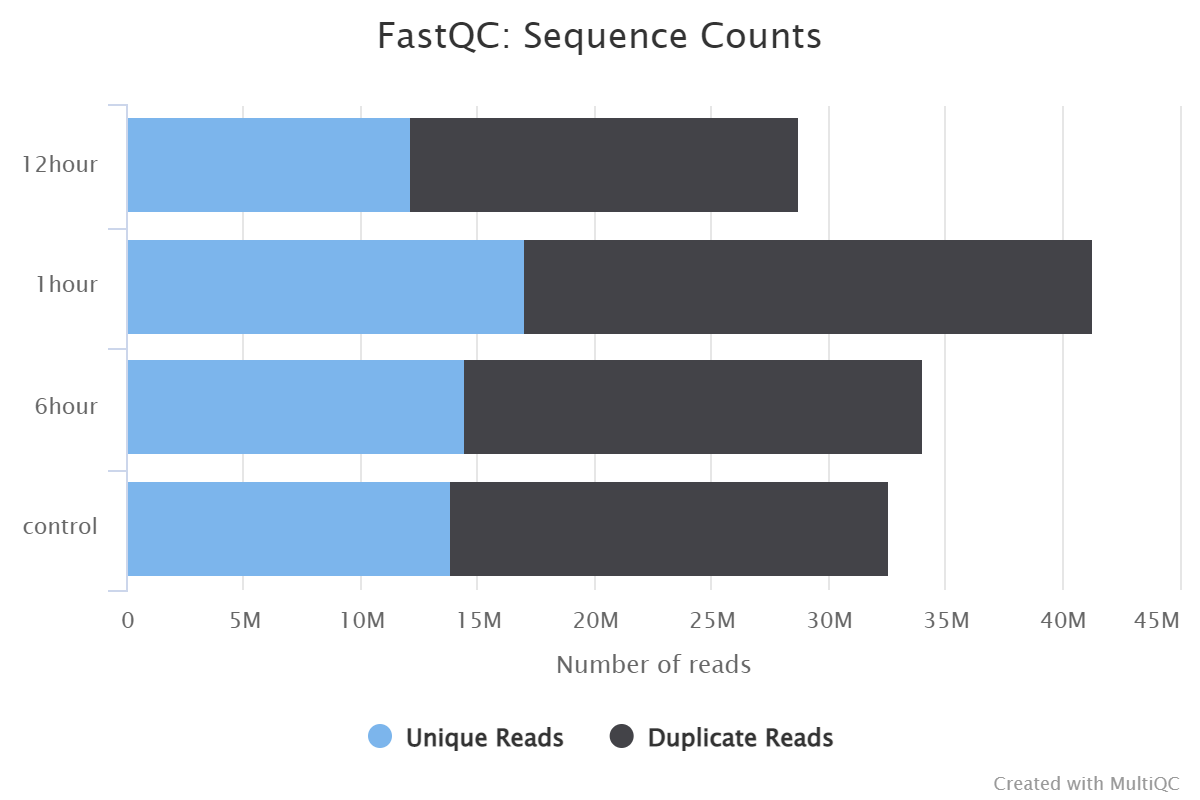
\includegraphics[width=1\textwidth]{fastqc_sequence_counts_plot}
    \caption{The number of reads for each sample, showing the proportion of duplicate reads.}
    \label{fig:fastqc_sequence_counts_plot}
\end{figure}
\newpage

The samples in \autoref{fig:fq_screen_plot} show no sign of contamination. There is an almost 100\% successful alignment to the human genome, with some alignment to other sequences which share genetic similarities. Some degree of multi-mapping (20\%) with the human reference is present. This may be caused by regions of low-complexity or by structural variants \citep{rhoads2015pacbio}

\begin{figure}[!h]
    \centering
    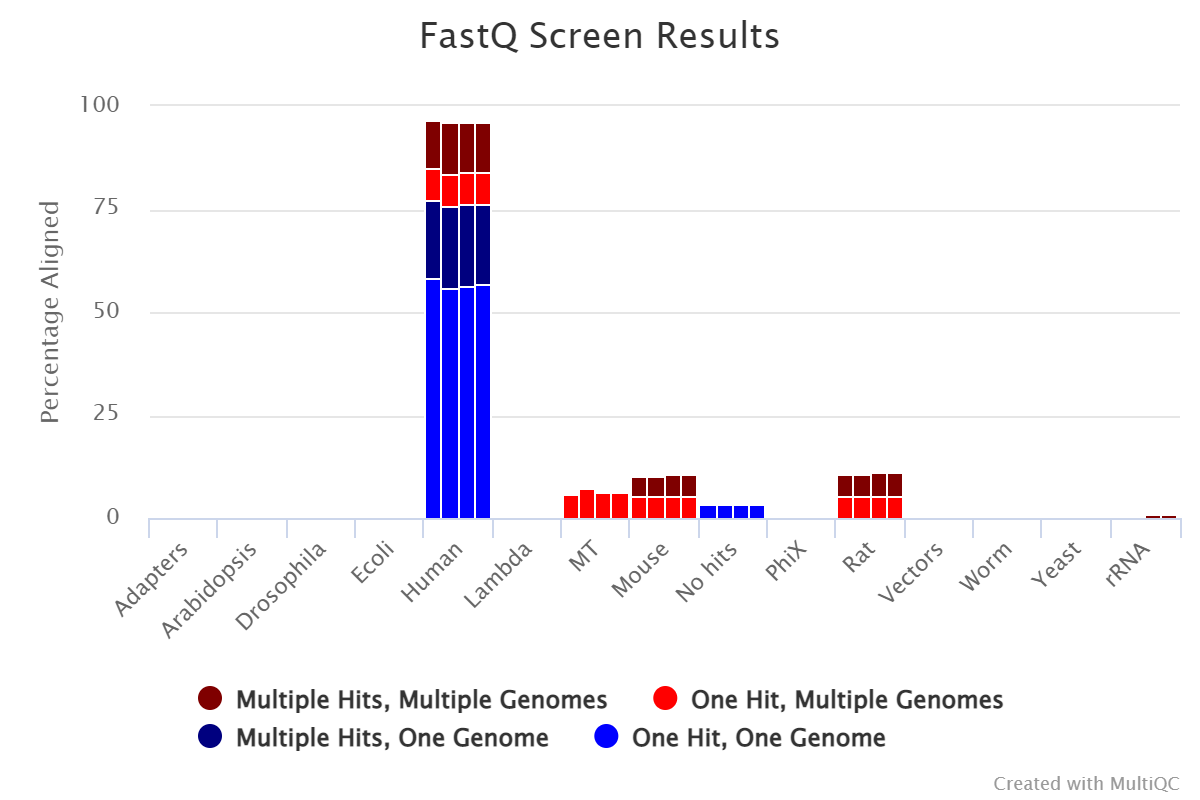
\includegraphics[width=1\textwidth]{fq_screen_plot}
    \caption{FastQ Screen plot showing the percentage of the reads aligned to which reference sequence(s).} 
    \label{fig:fq_screen_plot}
\end{figure}


\subsection{Preprocessing}
FastQC detected traces (<0.5\%) of TruSeq adapters in the FASTQ files, which is corroborated by the sequencer's manual \citep{HiSeq2000} stating that it makes use of the 'TruSeq family of reagents'. Adapter sequences were trimmed using CutAdapt (\autoref{fig:cutadapt_trimmed_sequences_plot_3}), and resultant reads shorter than 45 bp long were removed. Smaller reads lead to greater ambiguity during alignment as they have a greater probability of being multi-mapped.  The data was of good quality to begin with, so trimming had little overall effect on the reads, although the read lengths are no longer uniform.
%Between 1.3 and 1.6\% of all base-pairs were trimmed across the four samples. (why is this happening)


\begin{figure}[!h]
    \centering
    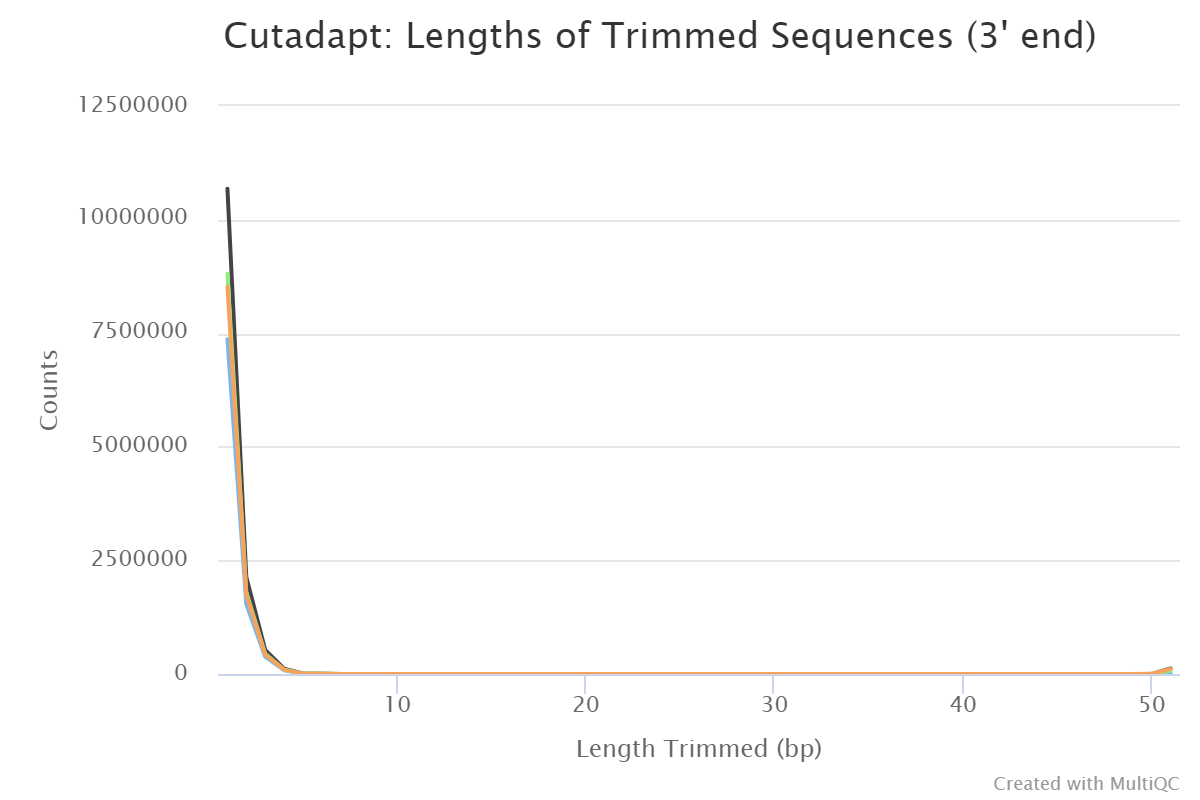
\includegraphics[width=1\textwidth]{cutadapt_trimmed_sequences_plot_3}
    \caption{The number of base-pairs trimmed per read from the 3' end.} 
    \label{fig:cutadapt_trimmed_sequences_plot_3}
\end{figure}
\newpage

MultiQC does not support Prinseq++ as of version 1.11, however its output reports are simple to interpret. They provide the number of reads filtered by \texttt{-lc\textunderscore dust} according to their DUST score (a measure of low complexity). These figures removed approximately 0.1\% of the total amount of reads for their respective sample. No reads were removed by \texttt{-ns\textunderscore max\textunderscore n} based on the number of \textit{N}'s.



\subsection{Read Alignment}
The removal of short reads and reads low in complexity has reduced ambiguity when aligning to a reference genome \citep{rhoads2015pacbio}. Nonetheless STAR experienced some degree of multimapping, shown in \autoref{fig:star_alignment_plot}. The number of loci \texttt{Nmap} a read maps to is stored in the generated BAM file as \texttt{NH:i:Nmap}. If \texttt{Nmap} exceeds a certain threshold (10 by default) it will be labelled as 'mapped to too many loci' and excluded from the final BAM file. This is the most significant filtering step so far, removing 16\% to 18\% of the total read counts. Despite the loss of this substantial chunk of our reads, the main causes \citep{rhoads2015pacbio} for multi-mapping have been mitigated where possible: 
\begin{itemize}
\item[] Low-complexity regions were filtered in the previous step using Prinseq++.
\item[] Structural variants, while frequent in cancer-derived transcriptomes, are bypassed in STAR's splice-aware algorithm \citep{Dobin2013}, allowing different parts of the same read to map to distant genomic loci (possibly to different strands or chromosomes).
\item[] Longer read lengths and paired-end reads should reduce multi-mapping, although these factors were immutable at this stage.
\end{itemize}


\begin{figure}[!h]
    \centering
    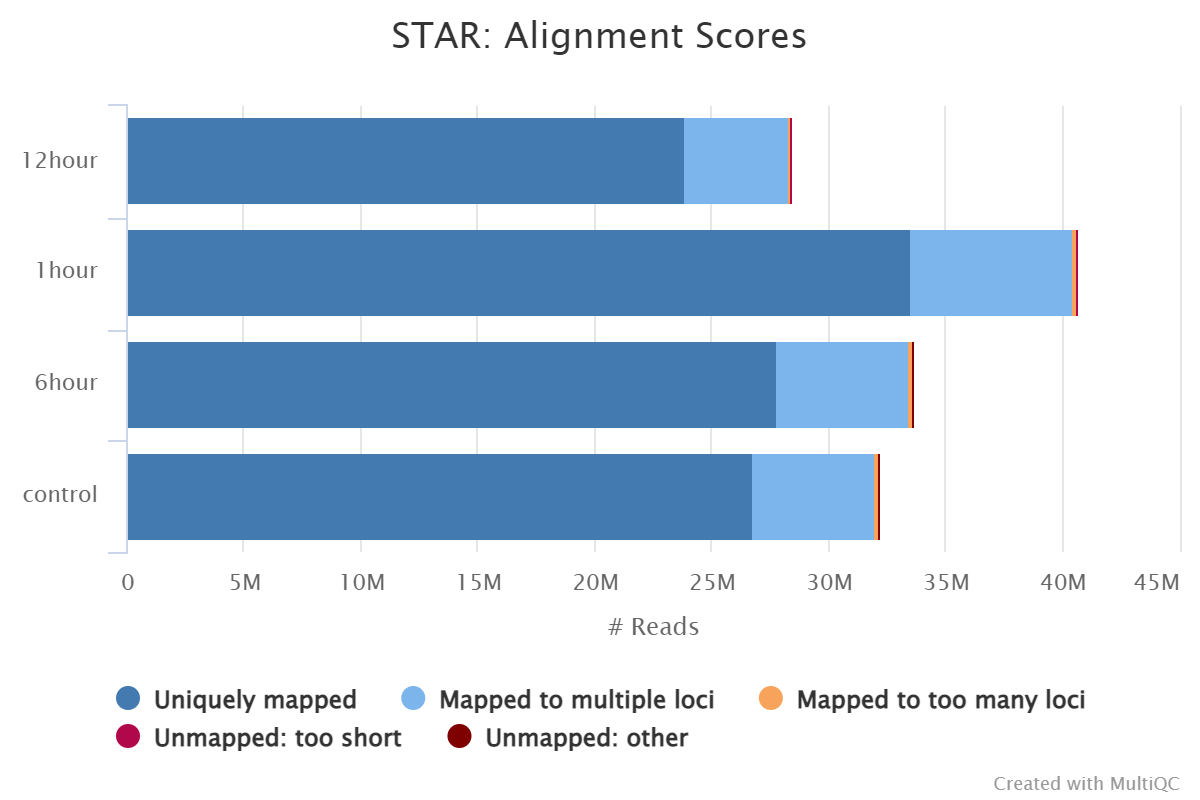
\includegraphics[width=1\textwidth]{star_alignment_plot}
    \caption{Number of uniquely mapped reads which passed all filters to the final BAM file, and the number of problematic reads which were consequently remained unaligned and were removed.} 
    \label{fig:star_alignment_plot}
\end{figure}
\newpage

%\subsection{Post-Alignment}
%At this stage tables containing information on the expected number of reads aligned to each gene are imported into R. Here we will be largely shifting our focus from the \textit{individual} reads, to \textit{collective} reads which align to each gene, i.e. to the expected read counts given in the tables produced through RSEM. The \ac{TMM} normalisation technique is performed, which adjusts the read count values per gene for confounding variables which are not biologically relevant. 

%Genes with low counts (<10) are removed as they can be considered as noise and are not expressed at any biologically meaningful level \citep{law2016rna}. These lowly expressed genes are particularly error-prone, and were shown to be highly sensitive to the \textit{in silico} methods used \citep{everaert2017benchmarking}.

\subsection{QC Summary}
The raw data in our starting FASTQ files was of good quality according to all tested metrics, resulting in Cutadapt and Prinseq++ having little effect on the read counts (\autoref{tab:read_counts}). Nonetheless a substantial portion of the reads suffered from multi-mapping and were excluded by the STAR aligner.

\begin{table}[!h]
\centering
\caption{The read counts in millions after passing through the processing tool indicated in the first column.}
\label{tab:read_counts}
\begin{tabular}{cclll}
\toprule
                                                                   & \textbf{Control} & \textbf{1 hour} & \textbf{6 hour} & \textbf{12 hour} \\ \midrule
Raw data                                       & 32.62M           & 41.30M          & 34.08M          & 28.77M           \\ 
\begin{tabular}[c]{@{}c@{}}Cutadapt\end{tabular} & 32.23M           & 40.81M          & 33.71M          & 28.54M           \\ 
\begin{tabular}[c]{@{}c@{}}Prinseq++ \end{tabular}    & 32.22M           & 40.75M          & 33.66M          & 28.50M           \\ 
\begin{tabular}[c]{@{}c@{}}STAR \end{tabular}        & 26.80M           & 33.54M          & 27.78M          & 23.89M           \\ \bottomrule
\end{tabular}
\end{table}


% The edgeR vignette suggests to use the raw counts (?) of RSEM for normalisation, as opposed to using the already normalised TPM so we went with this.
 % FPKM/RPKM are not good measures of relative abundance because the FPKM/RPKM of a transcript can change between two samples even if its relative abundance stays the same.
% https://groups.google.com/g/rsem-users/c/GRyJfEOK1BQ <- very good explanation 

%\subsection{Multiple testing Correction}
%FDR
%Benjamini Hochback 

\section{Post-Alignment Quality Control}
From this point forward we are mostly concerned with genes and the number of reads aligned to those genes in a tabular format, as opposed to individual unaligned reads. These were imported into R and converted into a \texttt{DGEList} object, \texttt{y}, consisting of multiple data-frames. The \texttt{y\$counts} dataframe initially contains the raw read count values for the four samples and a total of 60664 genes, each comprising a single row (\autoref{tab:gene_counts1}). 

In typical RNA-seq studies it is wise to search for potential batch effects and covariates, however with just a single replicate per condition it is impossible to distinguish such effects from real, biologically meaningful changes.

\begin{table}[h]
\centering
\caption{The first five out of a total 60664 rows of \texttt{y\$counts}. Notice the first two genes with low read counts which will be subsequently filtered }
\label{tab:gene_counts1}
\begin{tabular}{llllllll}
\toprule
\textbf{Genes}           & \textbf{1hr}     & \textbf{12hr}    & \textbf{6hr}     & \textbf{0hr}      \\ \midrule
ENSG00000000003 & 2       & 0       & 1       & 2        \\
ENSG00000000005 & 1       & 0       & 2       & 0        \\
ENSG00000000419 & 2491.7  & 1694.74 & 1703.4  & 1598.21  \\
ENSG00000000457 & 634.37  & 432.45  & 540.83  & 424.32   \\
ENSG00000000460 & 1176.63 & 1121.55 & 1415.17 & 1041.77  \\
...             & ...     & ...     & ...     & ... \\  \bottomrule
\end{tabular}
\end{table}

Of these 60664 genes, 43559 did not meet the minimum requirement of having at least 10 read counts for at least one sample, making them indistinguishable from noise and subsequently filtered. These counts were \ac{TMM} normalised, which did not affect the number of genes, but adjusted  read counts for between-sample differences \citep{robinson2010scaling}. The filtered and normalised data is represented holistically in \autoref{fig:boxplot_filtered}.


\begin{figure}[!h]
    \centering
    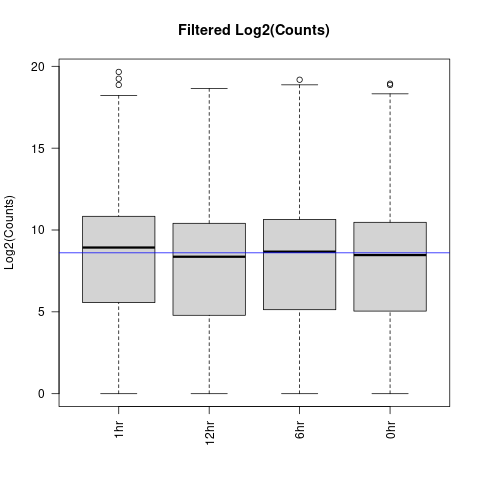
\includegraphics[width=10cm]{boxplot_filtered}
    \caption{Distribution of log$_2$-transformed counts per sample, including the control represented as '0hr'. The blue line bisecting the graph signifies the global median across all samples.} 
    \label{fig:boxplot_filtered}
\end{figure}
\clearpage

\section{Differential Gene Expression Analysis}
% Methods which compare values against a mean (e.g. Z-scores and MD-plots) are not particularly useful since we want to compare values against the control and not against the other samples
Using edgeR's classic approach \texttt{exactTest}, we compared the three treated samples (1hr, 6hr, 12hr) against the control which acted as a baseline. This generated a data frame with Ensembl gene IDs as row names, together with their respective \ac{logFC}, read counts per million, raw \textit{p}-value and \ac{FDR}. Here, the \ac{logFC} represents the \textit{magnitude} of the differential expression while the \ac{FDR} represents the \textit{significance} of the difference in expression. 

The \ac{FDR} is a form of an adjusted \textit{p}-value, applied to counteract the multiple comparisons problem arising from the hundreds of generated \textit{p}-values. This adjustment is common to RNA-seq analyses, although there is some disagreement in the literature whether it should be performed \citep{rothman1990no, streiner2011correction}, and to exercise caution when dealing with \textit{p}-values in general \citep{gardner1986confidence, greenland2016statistical, vidgen2016p}. In this study we followed the recommended edgeR procedure, using \ac{FDR}s in conjunction with the Benjamini-Hochberg controlling method \citep{benjamini1995controlling}. These values represent the probability of a type I error (i.e. a false positive result) for that specific gene. % fix this

% watch https://www.youtube.com/watch?v=K8LQSvtjcEo&ab_channel=StatQuestwithJoshStarmer

Threshold values of 1.5 for the \ac{logFC} and 0.05 for the \ac{FDR} were applied to define the truly differentially expressed genes in the data frame. With no possible objective justification of the appropriate thresholds, the choice was largely arbitrary. A \textit{p}-value cut-off of 0.05 (here, the \ac{FDR} acting as an adjusted \textit{p}-value) is a \textit{de facto} standard, popularised by Sir Ronald Fisher who stated it was "convenient to take this point as a limit in judging whether a deviation is to be considered significant or not" \citep{fisher1925statistical}. A standard \ac{logFC} cut-off does not exist, with similar studies using thresholds of anywhere between 0.5 and 2 \citep{zhao2018many, cardoso2019gene, handschuh2018gene}. One must bear in mind that this is a log$_2$ scale, and that negative values indicate a decrease in transcripts, e.g. a \ac{logFC} of -1.5 is equivalent to a third of the number of transcripts relative to the control. Absolute values are used in \ac{logFC}-based filtering to target both up- and down-regulation.

% If the phenolic treatment is successful in inducing differentiation, we should expect a divergence from a typically \ac{AML} transcriptome. The literature \citep{santos2000expression, mark2017transcriptomes} suggests that the cells will begin to exhibit monocytic or granulocytic characteristics, followed by apoptosis. This progression should be reflected in the activated JAK-STAT signaling pathway and the NF-$\kappa\beta$ pathways \citep{matikainen1997retinoic, gianni1997stat1, cohen2005jak, ren2013resveratrol, iwata2016parp9}. 



\subsection{Data Exploration}

A set of \ac{DEG}s was generated for each of the three time points, with considerable overlap between them represented as a Venn diagram in \autoref{fig:venn}. The 1hr sample shows a high proportion of uniquely expressed genes, and a higher overall number of \ac{DEG}s (\autoref{DEG_counts_barchart}). This is similarly reflected in the PCA plot, \autoref{fig:PCA_logFCs}, which shows the 1hr time point as an outlier, while the 6hr and 12hr points cluster closely. One potential hypothesis to explain this irregular spread of data is that the cells at the 1hr timepoint were in the process of differentiation and apoptosis, while the cells at 6hr and 12hr had reached a stable equilibrium, after the phenol-prone cells have died off.


\begin{figure}[!h]
    \centering
    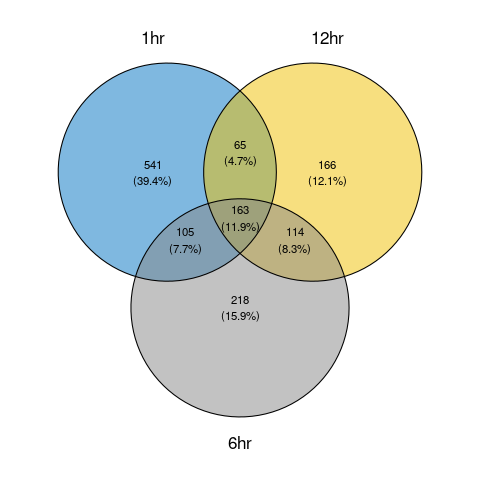
\includegraphics[width=9cm]{venn}
    \caption{Percentages of shared and unique \ac{DEG}s.} 
    \label{fig:venn}
\end{figure}

\begin{figure}[!h]
    \centering
    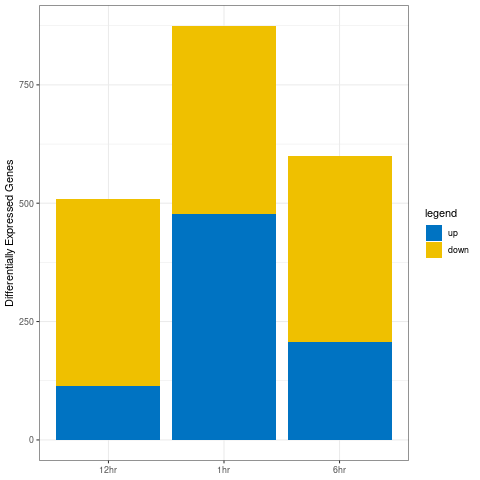
\includegraphics[width=10cm]{DEG_counts_barchart}
    \caption{Number of up- and down-regulated genes per experimental time-point.} 
    \label{fig:DEG_counts_barchart}
\end{figure}

\begin{figure}[!h]
    \centering
    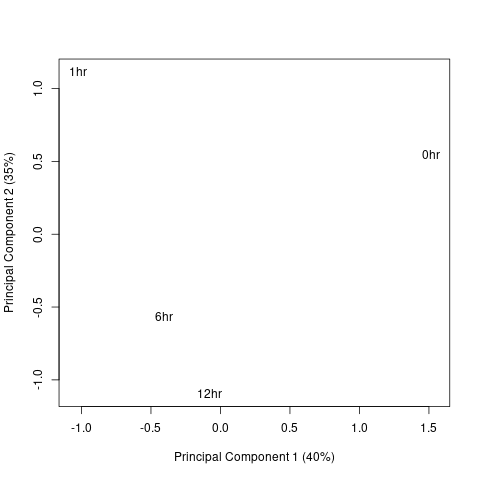
\includegraphics[width=8cm]{PCA_logFCs}
    \caption{PCA plot based on normalised counts.}
    \label{fig:PCA_logFCs}
\end{figure}
\clearpage
% Scree plot

% Bar chart of up/down for each time point

% Volcano plot
% Useful for volcano plots i think: https://huygens.science.uva.nl/VolcaNoseR/
% This too https://rdrr.io/bioc/vidger/man/vsVolcano.html


\subsection{Evaluation of Results}

We have cross-checked our resultant lists of \ac{DEG}s against a list of human housekeeping genes. These are essential to the biological function of the cell and should not change in expression levels, although exceptions to the rule exist \citep{khimani2005housekeeping}. Out of the 2833 housekeeping genes in the HRT Atlas \citep{hounkpe2021hrt}, one was found to be overly expressed in our results: ENSG00000105612. It codes for the DNase enzyme \textit{DNASE2} which plays a major role in apoptosis during foetal development \citep{yasuda1998structure}. 


\subsection{Biological Relevance of the Top DEGs}
The top 10 genes sorted by \ac{FDR}s from each of the three time points were selected for further biological investigation. The three lists were combined with considerable overlap into a single list of 17 genes, which are all protein-coding and have \ac{FDR}s of under 0.001 making them suitable candidates for further biological investigation. The \ac{FDR} was chosen for the sorting metric rather than the \ac{logFC} as it was deemed as a better indicator of biological relevance. The significance of the \ac{logFC} is tied to the role of the specific protein, i.e. a \ac{logFC} of 1.5 in a molecule with a cascading effect in a pathway may have a larger overall biological effect than a \ac{logFC} of 3 in a relatively benign molecule. The degree of up- or down-regulation of the 17 genes per time-point is shown in \autoref{heatmap_some}.

Comparing these results to the supplementary material provided by \cite{gatt2021tyrosol}, a study with particularly similar experimental design and goals, we find an overlap of 14 genes regulated the same direction. UTP14C, EGR3 and JAML were not found to be differentially expressed in \cite{gatt2021tyrosol}, while FOSB was found to be regulated but in the opposite direction.


\begin{figure}[!h]
    \centering
    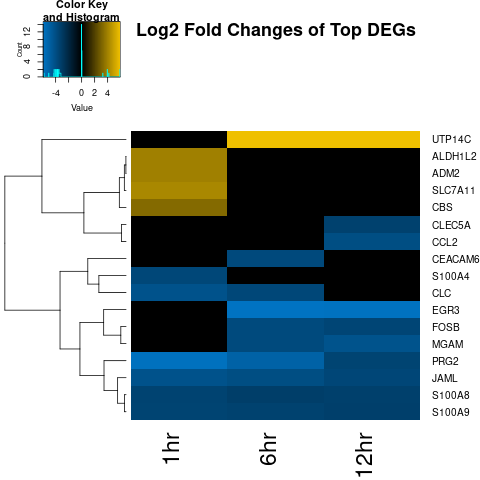
\includegraphics[width=8cm]{heatmap_some}
    \caption{The log$_2$ fold changes of the top differentially expressed genes sorted by their FDRs. The genes were originally in an ENSMBL transcript format but were translated to their gene symbol format.} 
    \label{fig:heatmap_some}
\end{figure}

% Table with FDRs and logFCs in appendix?
% write which were found in other studies


% List of DEGs from tyrosol study:  https://www.mdpi.com/2076-3417/11/21/10199
% Do the pathways make sense
% ENSG00000105612 housekeeping gene was found to be differentially expressed

% https://www.biostars.org/p/9510180/ reply says that even though a gene is downregulated, it might be suppressing other genes in the pathway which makes the other genes indirectly upregulated. Keep stuff like this in mind when interpreting gene expression.

\subsection{KEGG Pathway Visualisation}
Key KEGG pathways associated with the differentiation of \ac{AML} cells were visualised using Pathview, with \ac{DEG}s highlighted according to the direction of their regulation.



\subsection{Gene Set Enrichment Analysis}
Feeding genes in their Entrez format, and their \ac{logFC} values into the \texttt{gage} function, we have identified the significantly enriched gene sets in the form of \ac{GO} terms and \ac{KEGG} pathways. Apart from the aforementioned issue with a lack of replicates, these analyses come with a number of additional caveats, some inherent and others specific to this study:

\begin{itemize}
\item The BioStar handbook \citep{albert2020biostar} states that \ac{GO} analyses is that the results are moderately specific to the method used (this may seemingly be extended to include \ac{KEGG} pathways), with no existing objective method to validate the quality.
\item  Overlap between gene sets is possible, which may lead to some unexpectedly enriched sets. 
\item  GAGE reads genes as Entrez IDs, but our data was in the Ensembl format. Conversion was possible but imperfect since the conventions have slightly different definitions for each gene.
\item Gene sets are treated as separate entities, instead of as a part of an immensely complex and inter-connected biological system.
\end{itemize}

 %maybe find a better source for this
We have chosen a lenient FDR \textit{q}-score cut-off of 0.5, and suggest that these results be interpreted with caution. For comparison, the default GAGE cutoff was set at 0.1. \autoref{tab:gage} shows the concatenated results of the GAGE outputs for \ac{KEGG} pathways and \ac{GO} terms.


\begin{table}
\centering
\caption{Significantly enriched KEGG pathways and GO terms using a \textit{q}-value cut-off of 0.5. The \textit{Stat} column represents the generated GAGE statistic which indicates the magnitude and direction of the differential expression, analogous to the fold change in regular differentially expressed genes.}
\label{tab:gage}
\begin{tabular}{lllllll}
 \toprule
     \textbf{Gene Set} & \textbf{Term}                          & \textbf{Time} & \textbf{Stat}   & \textbf{\textit{p}-value} & \textbf{\textit{q}-value} & \textbf{\textit{N}}   \\ \midrule
            \textbf{KEGG}   \\ \midrule
hsa04145~ & phagosome                     & 1hr  & -1.963 & 0.035   & 0.039   & 10  \\
          &                               &      &        &         &         &     \\ \hline
hsa04380~ & osteoclast differentiation    & 1hr  & -1.864 & 0.039   & 0.039   & 12  \\
          &                               &      &        &         &         &     \\ \hline
hsa04380~ & osteoclast differentiation    & 6hr  & -1.882 & 0.039   & 0.039   & 13  \\
          &                               &      &        &         &         &     \\ \hline
hsa04620~ & toll-like receptor signaling~ & 12hr & -1.565 & 0.068   & 0.167   & 10  \\
          & pathway                       &      &        &         &         &     \\ \hline
hsa04145~ & phagosome                     & 12hr & -1.441 & 0.084   & 0.167   & 10  \\
          &                               &      &        &         &         &     \\ \hline
hsa04380~ & osteoclast differentiation    & 12hr & -1.136 & 0.135   & 0.180   & 12  \\
          &                               &      &        &         &         &     \\ \hline
hsa04062~ & chemokine signaling~          & 12hr & -0.454 & 0.327   & 0.327   & 11  \\
          & pathway                       &      &        &         &         &    \\ \midrule

            \textbf{GO term}   \\ \midrule
GO:0002376  & immune system process                  & 12hr & -1.998 & 0.024   & 0.408   & 67  \\
            &                                        &      &        &         &         &     \\ \hline
GO:0002376  & immune system process                  & 6hr  & -3.258 & 0.001   & 0.013   & 54  \\
            &                                        &      &        &         &         &     \\ \hline
GO:0006323~ & DNA packaging                          & 1hr  & 1.984  & 0.038   & 0.441   & 10  \\
            &                                        &      &        &         &         &     \\ \hline
GO:0006333  & ~chromatin assembly or~                & 1hr  & 1.984  & 0.038   & 0.441   & 10  \\
            & disassembly                            &      &        &         &         &     \\ \hline
GO:0006325~ & establishment, maintenance~       & 1hr  & 1.649  & 0.058   & 0.448   & 13  \\
            & of chromatin architecture                 &      &        &         &         &     \\ \hline
GO:0001775~ & cell activation                        & 1hr  & 1.181  & 0.125   & 0.472   & 13  \\
            &                                        &      &        &         &         &     \\ \hline
GO:0006520~ & amino acid metabolic            & 1hr  & 1.172  & 0.128   & 0.472   & 12  \\
            &     process                                   &      &        &         &         &     \\ \hline
GO:0006139  & ~nucleic acid metabolic ~ & 1hr  & 1.103  & 0.137   & 0.472   & 45  \\
            &    process   &      &        &         &         &     \\ \hline
GO:0006355  & ~regulation of transcription,~         & 1hr  & 1.075  & 0.144   & 0.472   & 27  \\
            & DNA-dependent                          &      &        &         &         &     \\ \hline
GO:0002376  & immune system process                  & 1hr  & -2.156 & 0.016   & 0.379   & 64  \\
            &                                        &      &        &         &         &    \\ \bottomrule
\end{tabular}
\end{table}

These gene set level results are not reflected in the literature \citep{matikainen1997retinoic, gianni1997stat1, cohen2005jak, ren2013resveratrol, iwata2016parp9}, which has repeatedly shown that the JAK-STAT signaling pathway and the NF-$\kappa\beta$ pathway play an essential role in differentiation of \ac{AML}, and are activated by differentiation agents. \cite{gatt2021tyrosol} found the \textit{Myeloid differentiation} \ac{GO} term (\ac{GO}:0030099) to be especially significant at an \ac{FDR} of 0.0001. Combined with the high \textit{q}-scores and the aforementioned caveats, interpretation of these results is difficult and only give a weak indication of the effectiveness of the treatment. 

Nevertheless, it is clear that overall the gene sets in \cite{tab:gage} somehow link to morphologically changing myeloid cells, particularly the \ac{GO} terms for the 1hr sample. The up-regulation of GO:0001775 is particularly indicative, which is defined\footnote{\url{https://gowiki.tamu.edu/wiki/index.php/Category:GO:0001775_!_cell_activation} (Last accessed 29/06/22)} as "a change in the morphology or behaviour of a cell resulting from exposure to an activating factor such as a cellular or soluble ligand."


%Pathview results

% good resource: https://ressources.france-bioinformatique.fr/sites/default/files/4%20-%20FGSA_Roscoff.pdf
% Resulting enriched pathways -> statistical probability rather than a biological certainty


\section{Summary}
\enlargethispage{\baselineskip} % so you do not get a single line in another page
